\subsection{FP2MP LLM-MAS Architecture}

The proposed method frames weakly structured problem solving as an \emph{iterative uncertainty reduction process} over a shared state space, rather than a single-shot artifact generation task.
Architecturally, the system is implemented as a computation graph (LangGraph) built on top of a three-level blackboard memory and controlled by a closed-loop \emph{decomposition--execution--curation--critique} cycle (see Figure \ref{figure:fp2mp_architecture}).
The architectural illustration was generated using generative AI tools (Google Gemini, Nano Banana, NotebookLM) based on an author-defined specification of the proposed system and was subsequently reviewed, edited, and validated by the authors.

\begin{figure}
    \centering
    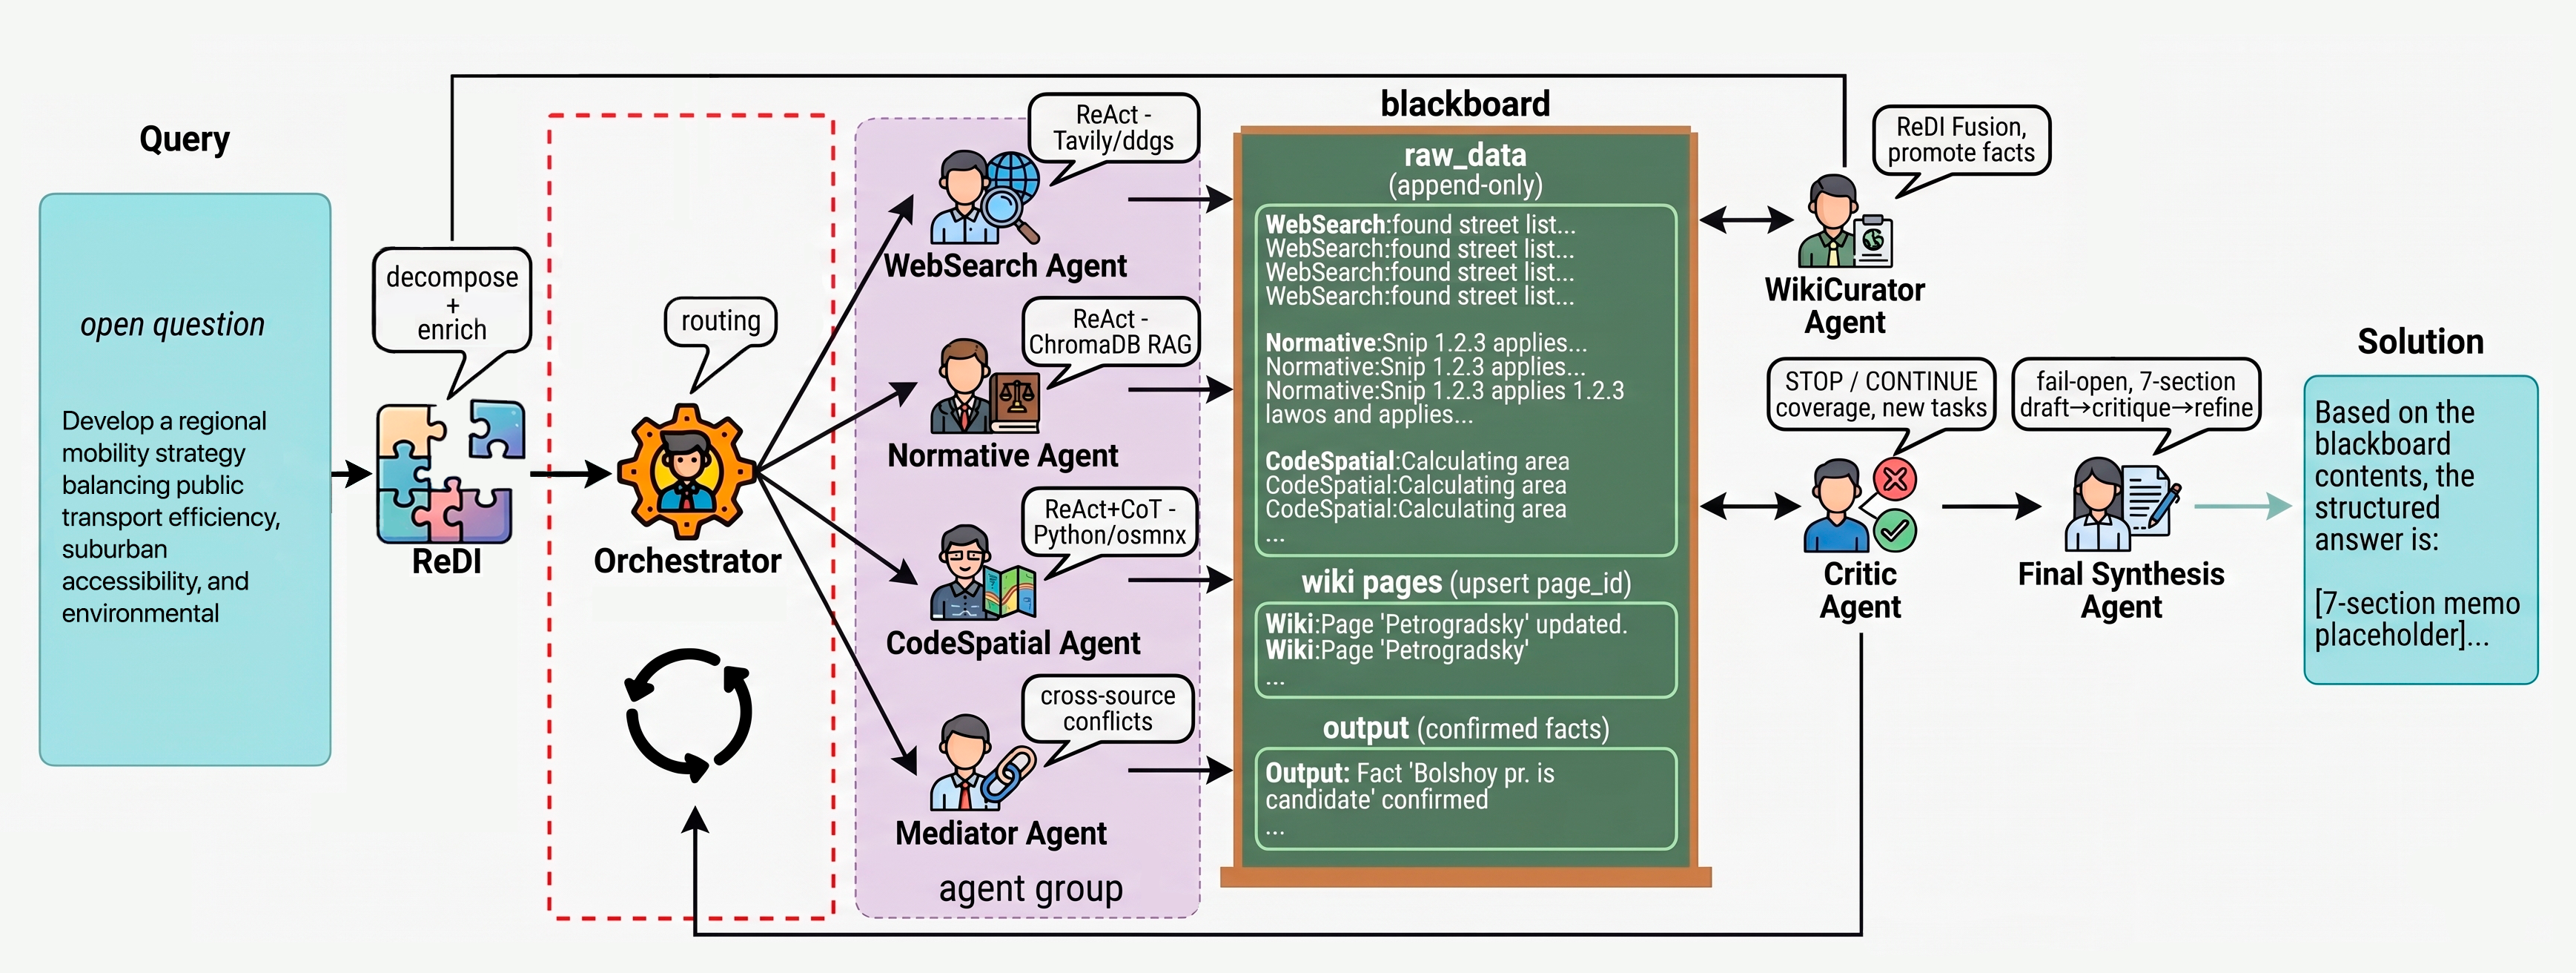
\includegraphics[width=1\linewidth]{Sections/3_methodology/Figures/fp2mp_architecture.png}
    \caption{Proposed FP2MP LLM-MAS architecture.}
    \label{figure:fp2mp_architecture}
\end{figure}

A key design principle is that the properties distinguishing LLM-based multi-agent systems (multi-agent coordination, reasoning, tool use, iterative refinement, aggregation, communication, and shared memory) are not treated as separate modules.
Instead, they emerge naturally from a unified graph structure.

\subsubsection{Query Decomposition (ReDI)}

Given an ill-defined problem $p$, the ReDI module decomposes it into a set of independent sub-queries:

\[
D(p) = \{(sq_i, m_i)\}_{i=1}^{k}, \qquad k \in [3,5],
\]

where each sub-query $sq_i$ is assigned an intent aspect and a modality hint $m_i \in \{\text{web},\,\text{normative},\,\text{code},\,\text{any}\}$.

During enrichment, each $sq_i$ is augmented with paraphrases, keywords, and domain-specific prompts to improve retrieval coverage.
Importantly, modality is used only as a \emph{routing context} rather than a strict constraint: final executor selection remains the responsibility of the orchestrator.

\subsubsection{Shared Memory (Blackboard)}

System state is represented as a three-level shared blackboard:

\[
B = (R, W, O),
\]

where:

\begin{itemize}
    \item $R$ — raw outputs log (\texttt{raw\_data}, append-only),
    \item $W$ — structured wiki-like knowledge pages (upsert by \texttt{page\_id}),
    \item $O$ — validated facts (upsert by \texttt{fact\_id}, conflict resolved by confidence).
\end{itemize}

Agents do not communicate directly.
Instead, they interact via read and write operations on the blackboard.
This design simultaneously implements shared memory and indirect communication, while allowing the solution path to evolve dynamically as new evidence is added.

\subsubsection{Orchestration and Specialized Agents}

The orchestrator performs capability-based routing.
Using structured capability cards (\texttt{handles}/\texttt{cannot\_do}), it assigns each sub-query to the most suitable agent via LLM-based reasoning.

Execution is parallelized (up to three dispatches per round), and failed tasks are re-routed if confidence drops below $0.4$ or an agent exceeds iteration limits.

The system includes the following specialized ReAct agents:

\begin{itemize}
    \item \textbf{WebSearchAgent}: web retrieval (Tavily/DDGS) and page extraction for factual queries.
    \item \textbf{NormativeAgent}: retrieval from a local ChromaDB-based normative index with web fallback.
    \item \textbf{CodeSpatialAgent}: Python-based execution for spatial and numerical reasoning (osmnx, geopandas, geopy).
\end{itemize}

The CodeSpatialAgent follows a strict pipeline:

\[
\text{HYPOTHESIS} \rightarrow \text{PLAN} \rightarrow \text{CODE} \rightarrow \text{EXECUTE} \rightarrow \text{INTERPRET},
\]

ensuring deterministic computation instead of textual approximation, which reduces spatial hallucinations.

\subsubsection{Curation, Aggregation, and Critique}

The \textbf{WikiCurator} acts as a fan-in aggregation node.
It transforms raw outputs into structured wiki pages and performs \emph{ReDI Fusion}, which includes:

\begin{itemize}
    \item deduplication via Jaccard similarity,
    \item keyword-overlap-based reranking,
    \item promotion of reliable statements into validated facts.
\end{itemize}

A fact $f$ is promoted into $O$ if:
\[
\mathrm{conf}(f) > \tau \; (\tau = 0.65)
\quad \text{or} \quad
|\mathrm{sources}(f)| \ge 2.
\]

The \textbf{MediatorAgent} performs cross-source synthesis, identifying agreements and contradictions.
The \textbf{CriticAgent} evaluates coverage of sub-queries and decides between $STOP$ and $CONTINUE$, optionally injecting missing tasks.
Termination occurs when all sub-queries are covered or a maximum iteration limit $T_{\max}$ is reached.

The system transition is defined as:

\[
B_{t+1} = \mathrm{Curator}\!\big(\mathrm{Agents}(\mathrm{Orch}(B_t))\big),
\]

with stopping condition:

\[
\mathrm{Critic}(B_t)=\text{stop}.
\]

\subsubsection{Final Synthesis (Fail-Open Mode)}

After termination, the system produces a final answer in \emph{fail-open} mode: it always outputs a concrete decision (e.g., choice, location, numeric value, or recommendation) instead of deferring with uncertainty.

The synthesis is based on weighted aggregation of validated facts and source agreement.
Reasoning quality is ensured via a three-pass $\text{DRAFT} \rightarrow \text{CRITIQUE} \rightarrow \text{REFINE}$ pipeline. The final output is structured as a seven-section expert memo:

\begin{enumerate}
    \item directed answer,
    \item problem framing,
    \item key dependencies,
    \item alternatives,
    \item justification,
    \item residual uncertainty,
    \item self-reflection.
\end{enumerate}